\subsection{Data Processing Pipeline}

We adopt the clinical motion capture dataset of Van Criekinge et al.~\cite{vancriekinge2023dataset} (ages 21--86) and convert the marker recordings into a HumanML3D-compatible skeletal graph format~\cite{guo2022generating}. This is achieved through SMPL body-model fitting~\cite{mahmood2019amass} and subsequent feature extraction.
During preprocessing, we resolved dataset-specific artifacts, including sensor measurement errors, initialization transients, mislabeled markers, and systematic coordinate axis misalignments. We discarded irreparably polluted clips (such as those exhibiting T-pose misclassifications or sub-threshold sequence lengths).

To ensure biological fidelity is preserved, we utilize a modified optimization pipeline adapted from VPoser~\cite{pavlakos2019expressivebodycapture3d}.
We formulated a frame-by-frame minimum-loss optimization using the L-BFGS engine.
Crucially, we implemented a multi-step pipeline where a local minimum is found \textit{before} the optimizer considers body pose priors and spatiotemporal consistency. This careful staging ensures that minor, individual biomechanical details are preserved during fitting without being overwhelmed by standard generic priors.
As shown in Fig.~\ref{fig:artifact}, standard priors induce crouch artifacts (left) and naive mapping causes mesh inflation (right); our optimized pipeline effectively mitigates these issues to recover a natural posture (center).

\begin{figure}[H]
	\centering
	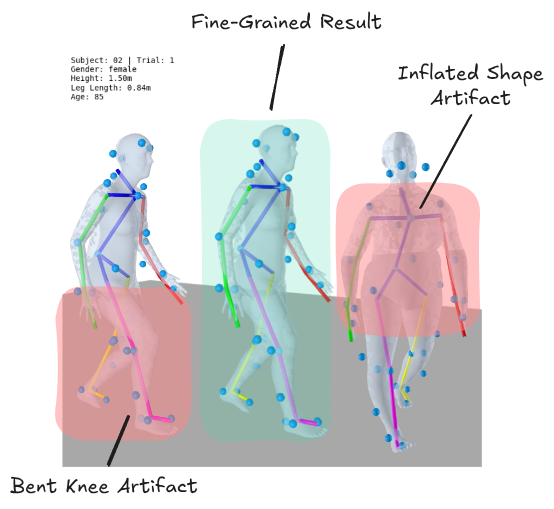
\includegraphics[width=0.7\linewidth]{sec/figs/BodyArtifacts.png}
	\caption{Artifact analysis in clinical motion retargeting.}
	\label{fig:artifact}
\end{figure}

\subsection{Age Classification Network}

To capture the biomechanical signatures of aging, we employ an age classifier built on a Spatial-Temporal Graph Convolutional Network (ST-GCN)~\cite{yan2018stgcn}. The network is fine-tuned to classify motion clips into three distinct age groups: Young ($<$35), Mid-age (35--60), and Elderly ($\geq$60).
By training the ST-GCN to successfully predict age groups from walking motions alone, the network learns to isolate demographic kinematic differences from general gait mechanics.

\subsection{Age-Conditioned Generative Network}

For motion synthesis, we leverage a conditional Motion Diffusion Model (MDM)~\cite{tevet2023human} capable of generating text-driven human motion.
Given the limited compute available for this proof-of-concept and the comparatively small size of our domain-specific dataset, end-to-end retraining of MDM is impractical and would also risk overwriting the strong text-to-motion prior already learned on HumanML3D.
We therefore adapt the pre-trained MDM using Low-Rank Adaptation (LoRA)~\cite{hu2022lora}, following the recipe of Sawdayee et al.~\cite{sawdayee2025dance}, to accept discrete age-group tokens. This provides a highly parameter-efficient mechanism to condition generation on specific demographic groups while keeping the underlying motion prior intact.

\subsection{Gait-Analysis Metrics for Evaluation}

To rigorously evaluate whether aging signals are preserved in the processed dataset and successfully reproduced by our generative model, we utilize standard, training-free gait-analysis metrics derived from clinical literature~\cite{bailey2023smartwatch, galasso2024development}:

\begin{itemize}
    \item \textbf{Spatiotemporal Parameters:} We compute the average walking speed, stride length, and cadence using heel-strike events detected via zero-velocity crossings of the ankle joints.
    \item \textbf{Gait Variability:} The consistency of a subject's gait is quantified using the Coefficient of Variation (CV) for both stride time and stride length, defined as:
    \begin{equation}
        \mathrm{CV} = \left( \frac{\sigma}{\mu} \right) \times 100\%
    \end{equation}
    where $\sigma$ is the standard deviation and $\mu$ is the mean of the parameter across steps.
    \item \textbf{Joint Range of Motion (RoM):} We measure the peak flexion and extension angles of the hip and knee joints during the gait cycle.
\end{itemize}

These metrics are computed deterministically on both the real ground-truth clips and the generated motion clips to provide a quantitative, biomechanically grounded evaluation.
